% Paquets généraux
\documentclass[a4paper,12pt,titlepage]{article}
\usepackage[T1]{fontenc}
\usepackage[utf8]{inputenc}
\usepackage[french]{babel}
\usepackage[gen]{eurosym}
%\usepackage[dvips]{graphicx}
\usepackage{fancyhdr}
\usepackage{pdfpages} 
\usepackage{multido}
\usepackage{hyperref}
%\usepackage{textcomp}
%\usepackage{aeguill}
\usepackage{schemabloc}
\usepackage[bitstream-charter]{mathdesign}
\usepackage{pstricks}
\usepackage{helvet}

\newcommand{\id}{54}
\newcommand{\nom}{Liaisons mécaniques}
\newcommand{\sequence}{04}
\newcommand{\num}{01}
\newcommand{\type}{TP}
\newcommand{\descrip}{Modélisation d'un solide. Comportement des liaisons mécaniques. Modéliser les mécanismes du laboratoire par un schéma cinématique, paramétré.}
\newcommand{\competences}{A3-C4: Analyse d'architecture et de comportement \\ &  Mod1-C1: Isolement d'un solide ou d'un système de solides \\ &  Mod2-C10-1: Modèle de solide indéformable \\ &  Mod2-C11: Modélisation géométrique et cinématique des mouvements entre solides indéformables \\ &  Mod2-C12: Modélisation cinématique des liaisons entre solides \\ &  Mod2-C15: Modélisation des actions mécaniques \\ &  Rés-C6: Utilisation d'un solveur ou d'un logiciel multi physique \\ &  Com1-C1: Différents descripteurs introduits dans le programme \\ &  Com2-C4: Outils de communication}
\newcommand{\nbcomp}{9}
\newcommand{\systemes}{Plateforme Stewart}
\newcommand{\systemessansaccent}{Plateforme Stewart}
\newcommand{\ilot}{2}
\newcommand{\ilotstr}{02}
\newcommand{\dossierilot}{\detokenize{Ilot_02 Plateforme Stewart}}
\newcommand{\imageun}{Plateforme}

\newcommand{\urlsysteme}{\href{https://www.costadoat.fr/systeme/57}{Ressources système}}
\newcommand{\matlabsimscape}{\href{https://github.com/Costadoat/Sciences-Ingenieur/raw/master/Systemes/Plateforme Stewart/Plateforme_Stewart_Simscape.zip}{Modèle Simscape}}
\newcommand{\solidworks}{\href{https://github.com/Costadoat/Sciences-Ingenieur/raw/master/Systemes/Plateforme Stewart/Plateforme_Stewart_Solidworks.zip}{Modèle Solidworks}}
\newcommand{\edrawings}{\href{https://github.com/Costadoat/Sciences-Ingenieur/raw/master/Systemes/Plateforme Stewart/Plateforme_Stewart.EASM}{Modèle eDrawings}}
\newcommand{\test}{Stewart_param1}
\newcommand{\testi}{Stewart_param2}
\newcommand{\testii}{Stewart_param3}
\newcommand{\testiii}{Stewart_param4}
\newcommand{\testiiii}{Stewart_euler}

\newcommand{\auteurun}{Renaud Costadoat}
\newcommand{\institute}{Lycée Dorian}


\usepackage{color}
\usepackage{xcolor}
\usepackage{colortbl}
\usepackage{helvet}
\renewcommand{\familydefault}{\sfdefault}
\usepackage{amsfonts}
\usepackage{amsmath}
%\usepackage{xspace}
\usepackage{varioref}
\usepackage{tabularx}
%\usepackage{floatflt}
\usepackage{graphics}
\usepackage{wrapfig}
\usepackage{textcomp}
\usepackage{tikz}
\usepackage{wrapfig}
\usepackage{gensymb}
\usepackage[european]{circuitikz}
\usetikzlibrary{babel}
\usepackage{ifthen}
\usepackage{cancel}
\usepackage{etoolbox}
\usepackage{multirow}
%\usepackage{boxedminipage}
\definecolor{gris25}{gray}{0.75}
\definecolor{bleu}{RGB}{18,33,98}
\definecolor{bleuf}{RGB}{42,94,171}
\definecolor{bleuc}{RGB}{231,239,247}
\definecolor{rougef}{RGB}{185,18,27}
\definecolor{rougec}{RGB}{255,188,204}%255,230,231
\definecolor{vertf}{RGB}{103,126,82}
\definecolor{vertc}{RGB}{220,255,191}
\definecolor{forestgreen}{rgb}{0.13,0.54,0.13}
\definecolor{blcr}{rgb}{0.59,0.69,0.84}
\definecolor{blfr}{rgb}{0.32,0.51,0.75}
\definecolor{orfr}{rgb}{0.90,0.42,0.15}
\definecolor{orcr}{rgb}{0.90,0.65,0.50}
\definecolor{orangef}{rgb}{0.659,0.269,0.072}
\definecolor{orange}{rgb}{0.58,0.35,0.063}
\definecolor{orangec}{rgb}{0.43,0.32,0.25}
\definecolor{rcorrect}{rgb}{0.6,0,0}
\definecolor{sequence}{rgb}{0.75,0.75,0.75}
\definecolor{competences}{rgb}{0.61,0.73,0.35}
\definecolor{grisf}{HTML}{222222}
\definecolor{grisc}{HTML}{636363}
\definecolor{normal}{HTML}{4087c4}
\definecolor{info}{HTML}{5bc0de}
\definecolor{success}{RGB}{92,184,92}
\definecolor{warning}{RGB}{240,173,78}
\definecolor{danger}{RGB}{217,83,79}
\hypersetup{                    % parametrage des hyperliens
    colorlinks=true,                % colorise les liens
    breaklinks=true,                % permet les retours à la ligne pour les liens trop longs
    urlcolor= blfr,                 % couleur des hyperliens
    linkcolor= orange,                % couleur des liens internes aux documents (index, figures, tableaux, equations,...)
    citecolor= forestgreen                % couleur des liens vers les references bibliographiques
    }

% Mise en page
\pagestyle{fancy}

\setlength{\hoffset}{-18pt}

\setlength{\oddsidemargin}{0pt} 	% Marge gauche sur pages impaire2s
\setlength{\evensidemargin}{0pt} 	% Marge gauche sur pages paires
\setlength{\marginparwidth}{00pt} 	% Largeur de note dans la marge
\setlength{\headwidth}{481pt} 	 	% Largeur de la zone de tête (17cm)
\setlength{\textwidth}{481pt} 	 	% Largeu\textbf{r de la zone de texte (17cm)
\setlength{\voffset}{-18pt} 		% Bon pour DOS
\setlength{\marginparsep}{7pt}	 	% Séparation de la marge
\setlength{\topmargin}{-30pt} 		% Pas de marge en haut
\setlength{\headheight}{55pt} 		% Haut de page
\setlength{\headsep}{20pt} 		% Entre le haut de page et le texte
\setlength{\footskip}{30pt} 		% Bas de\textbf{ page + séparation
\setlength{\textheight}{700pt} 		% Hauteur de l'icone zone de texte (25cm)
\setlength\fboxrule{1 pt}
\renewcommand{\baselinestretch}{1}
\setcounter{tocdepth}{1}
\newcommand{\cadre}[2]
{\fbox{
  \begin{minipage}{#1\linewidth}
   \begin{center}
    #2\\
   \end{center}
  \end{minipage}
 }
}

\newcommand{\reponse}[1][4]
{
\multido{}{#1}
{\begin{center}\makebox[0.9\linewidth]{}  \\
\begin{center}\makebox[0.9\linewidth]{\dotfill} \\ \end{center}
}}

\newcommand{\titre}[1]
{\begin{center}
\cadre{0.8}{\huge #1} 
\end{center}
}


% En tête et pied de page
\lhead{\nom}
\rhead{
\includegraphics[width=2cm]{../../img/logo}}
\lfoot{Renaud Costadoat}
\cfoot{Page \thepage}

\fancypagestyle{correction}{%
  \fancyhf{}
  \lhead{\colorbox{danger}{\begin{minipage}{0.65\paperwidth} \textcolor{white}{\textbf{Correction}} \end{minipage}} }
  \rhead{
\includegraphics[width=2cm]{../../img/logo}}
  \lfoot{Renaud Costadoat}
  \rfoot{\colorbox{danger}{\begin{minipage}{0.6\paperwidth} \begin{flushright}\textcolor{white}{\textbf{Correction}}\end{flushright} \end{minipage}} }}

\renewcommand{\footrulewidth}{0.4pt}

\usepackage{eso-pic}
\newcommand{\BackgroundPic}{%
\put(0,0){%
\parbox[b][\paperheight]{\paperwidth}{%
\vfill
\begin{center}
\hspace{0.5cm}\vspace{0.5cm}

\includegraphics[width=\paperwidth,height=\paperheight,%
keepaspectratio]{../../img/fond3}%
\end{center}
\vfill
}}}

\newcommand{\BackgroundPicdeux}{%
\put(25,-30){%
\parbox[b][\paperheight]{\paperwidth}{%
\vfill
\begin{center}

\includegraphics[width=\paperwidth,height=\paperheight,%
keepaspectratio]{../../img/fond4}%
\end{center}
\vfill
}}}

\begin{document}

\AddToShipoutPicture{\BackgroundPicdeux}

\pagestyle{fancy}

\section{Le manège à sensations XXL}

Le système étudié ici est un manège appelé \og Manège à sensations XXL \fg. L'étude consiste à déterminer l'accélération subite par une personne, et de vérifier que la limite supportable (sans déconfort) par l'homme d'une valeur de 2g n'est pas dépassée...

\begin{figure}[htbp]
\begin{minipage}[c]{.48\linewidth}
\begin{center}
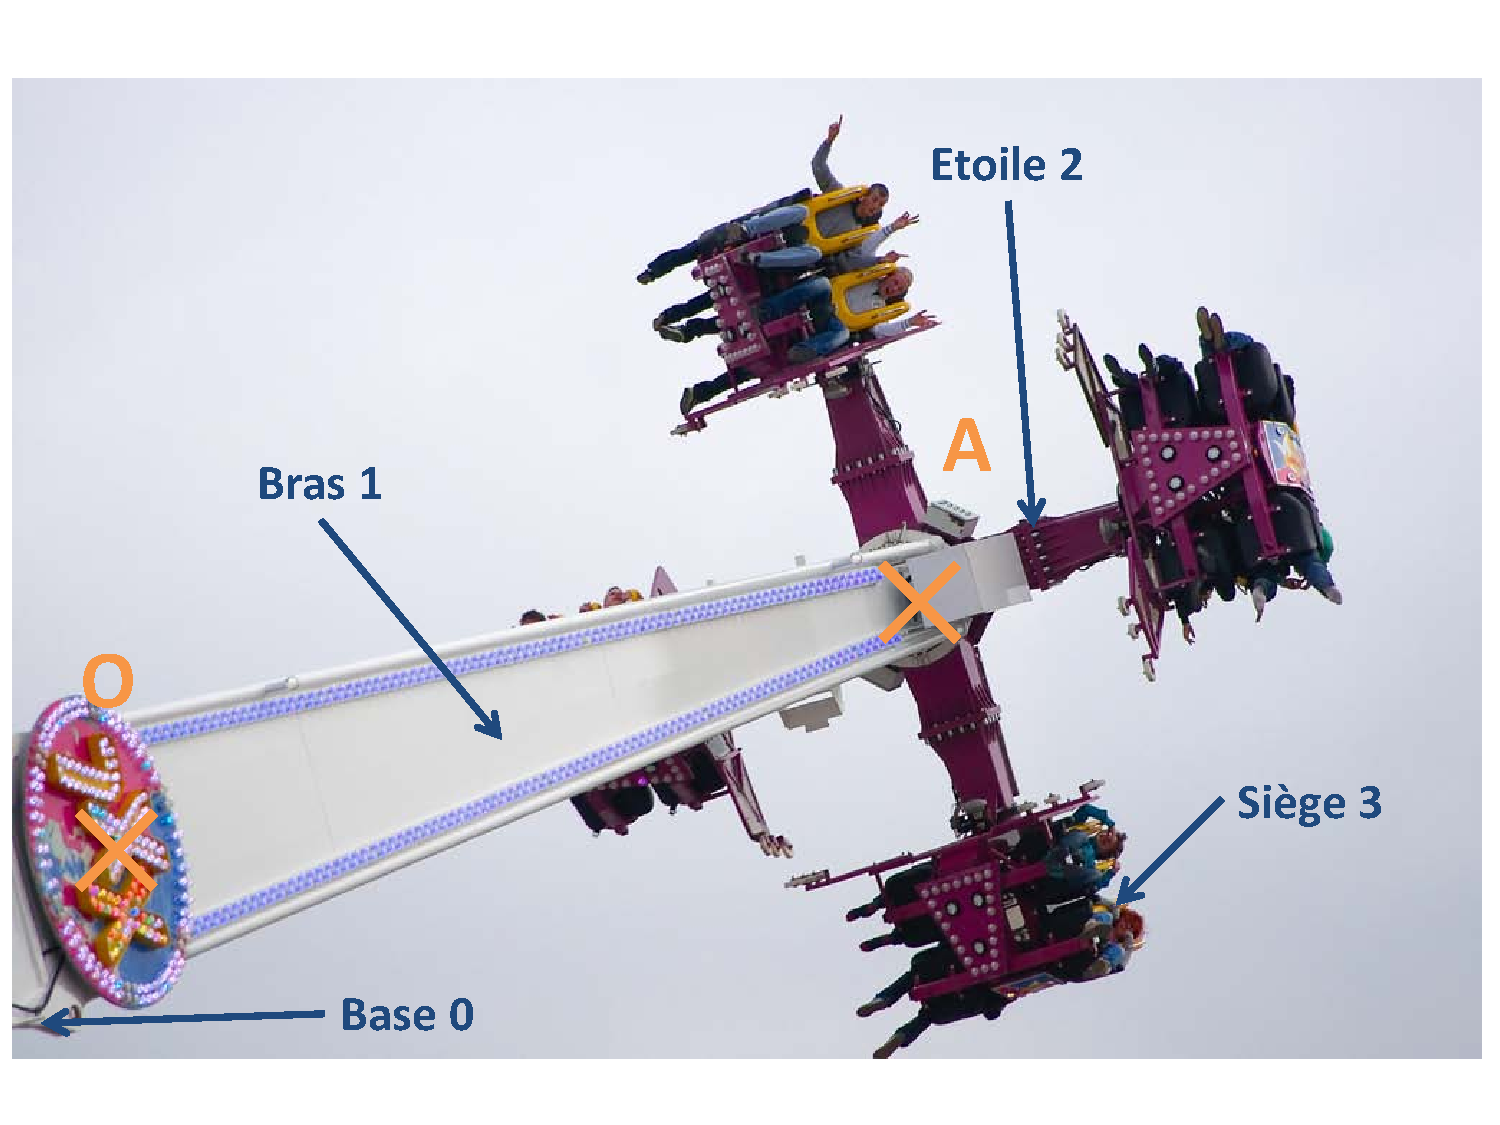
\includegraphics[width=\linewidth]{img/Manege1.pdf}
\caption{Vue du bras du ménège}
\label{fig:image1}
\end{center}
\end{minipage}
\hfill
\begin{minipage}[c]{.48\linewidth}
\begin{center}
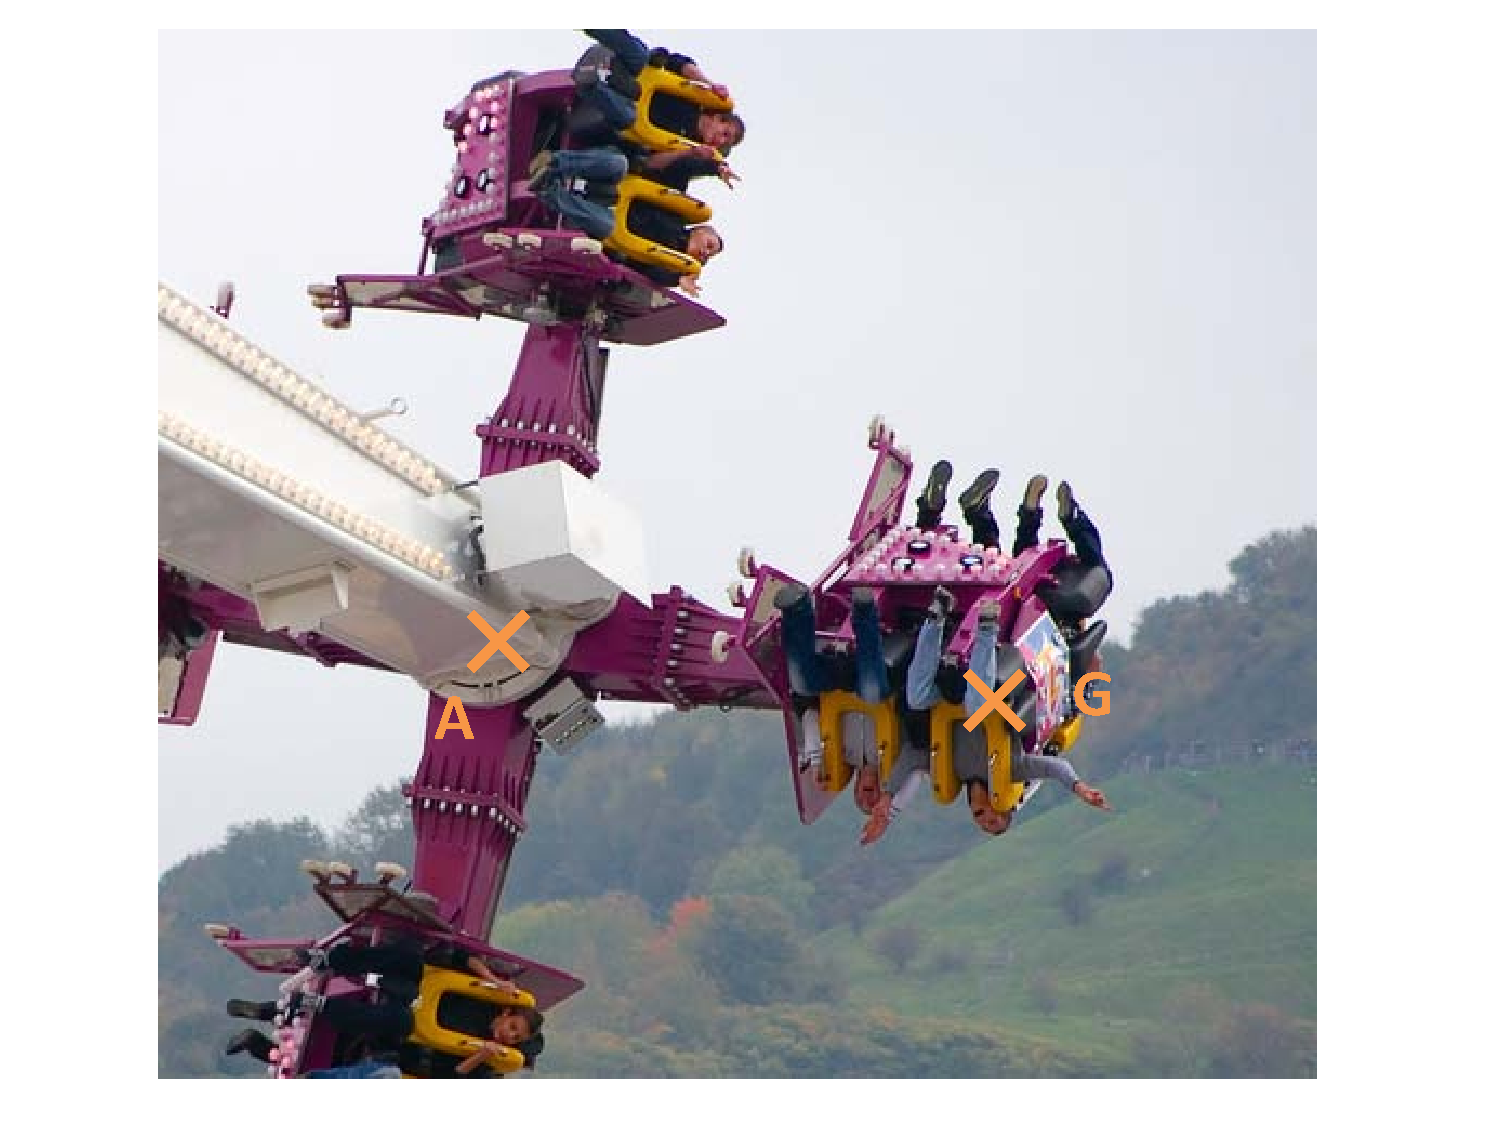
\includegraphics[width=\linewidth]{img/Manege2.pdf}
\caption{Vue de l'étoile}
\label{fig:image2}
\end{center}
\end{minipage}
\end{figure}

Ce système est constitué de quatre solides :
\begin{itemize}
 \item  La Base 0, de repère associé $R_O(\overrightarrow{x_0},\overrightarrow{y_0},\overrightarrow{z_0})$, fixe par rapport à la terre telle que l'axe $(O, \overrightarrow{z_0})$, soit dirigé suivant la verticale ascendante,
 \item Le Bras 1, de repère associé $R_1(\overrightarrow{x_1},\overrightarrow{y_1},\overrightarrow{z_1})$, en mouvement de rotation, d'axe $(O, \overrightarrow{x_0})$ par rapport à l base et tel que $\alpha=(\overrightarrow{y_0},\overrightarrow{y_1})=(\overrightarrow{z_0},\overrightarrow{z_1})$,
 \item L'étoile 2, de repère associé $R_2(\overrightarrow{x_2},\overrightarrow{y_2},\overrightarrow{z_2})$, en mouvement de rotation d'axe $(A, \overrightarrow{z_1})$ par rapport au plateau 1 tel que $\overrightarrow{OA}=a.\overrightarrow{z_1}$ (avec a constant), et $\beta=(\overrightarrow{x_1},\overrightarrow{x_2})=(\overrightarrow{y_1},\overrightarrow{y_2})$,
 \item Le siège 3 (lié à la personne, de repère associé $R_3(\overrightarrow{x_3},\overrightarrow{y_3},\overrightarrow{z_3})$, en mouvement de rotation d'axe $(A, \overrightarrow{x_2})$, avec $\gamma=(\overrightarrow{y_2},\overrightarrow{y_3})=(\overrightarrow{z_2},\overrightarrow{z_3})$
 \item La position de la personne est définie par son centre de gravité G, qui appartient au siège 3 et avec $\overrightarrow{AG}=b.\overrightarrow{x_2}+c.\overrightarrow{z_3}$ (avec b et c constants).
\end{itemize}

Seul le mouvement de rotation du bras 1 par rapport à la base 0 sera considéré.

\paragraph{Question 1:} Dans un premier temps, l'étude portera sur un mouvement dont l'accélération sera de la forme:

\begin{itemize}
 \item Pour $0 \le t \le t_0$ : $\ddot{\theta(t)}=\ddot{\theta_0}.sin(\frac{\pi.t}{t_0})$,
 \item Pour $t_0 \le t \le t_0+T$ : $\ddot{\theta(t)}=0$,
 \item Pour $t_0+T \le t \le 2.t_0+T$ : $\ddot{\theta(t)}=-\ddot{\theta_0}.sin(\frac{\pi}{t_0}(t-(t_0+T)))$,
 \item Les conditions initiales étant: $\dot{\theta(0)}=0$ et $\theta(0)=0$. $\ddot{\theta_0}$ est une constante.
\end{itemize}

Tracer:
\begin{itemize}
 \item l'accélération $\ddot{\theta(t)}$ en fonction du temps (t),
 \item la vitesse $\dot{\theta(t)}$ en fonction du temps (t),
 \item la position $\theta(t)$ en fonction du temps (t).
\end{itemize}

\newpage

\paragraph{Question 2:} Dans un second temps, la valeur pilotée sera la vitesse, elle sera de la forme:

\begin{itemize}
 \item Pour $0 \le t \le t_0$ : $\dot{\theta(t)}=\frac{\dot{\theta_0}}{t_0}.t$,
 \item Pour $t_0 \le t \le t_0+T$ : $\dot{\theta(t)}=\dot{\theta_0}$,
 \item Pour $t_0+T \le t \le 3.t_0+T$ : $\dot{\theta(t)}=-\frac{\dot{\theta_0}}{2.t_0}.t+\frac{\dot{\theta_0}}{2.t_0}.(T+3.t_0)$,
 \item Les conditions initiales étant: $\dot{\theta(0)}=0$ et $\theta(0)=0$. $\dot{\theta_0}$ est une constante.
\end{itemize}

Tracer:
\begin{itemize}
 \item la vitesse $\dot{\theta(t)}$ en fonction du temps (t),
 \item l'accélération $\ddot{\theta(t)}$ en fonction du temps (t),
 \item la position $\theta(t)$ en fonction du temps (t).
\end{itemize}

\newpage

\section{Camion benne}

Un camion à benne basculante ou camion benne est un type de camion utilisé généralement pour le transport de matériaux en vrac tel que du sable, du gravier, de terre ou de gravats.

Un camion à benne basculante est ordinairement équipé d'un vérin hydraulique qui soulève l'avant de la benne à la demande, permettant ainsi de la vider par gravité, en partie ou totalité, que le camion soit immobile ou en déplacement.

\begin{figure}[htbp]
\begin{minipage}[c]{.48\linewidth}
\begin{center}
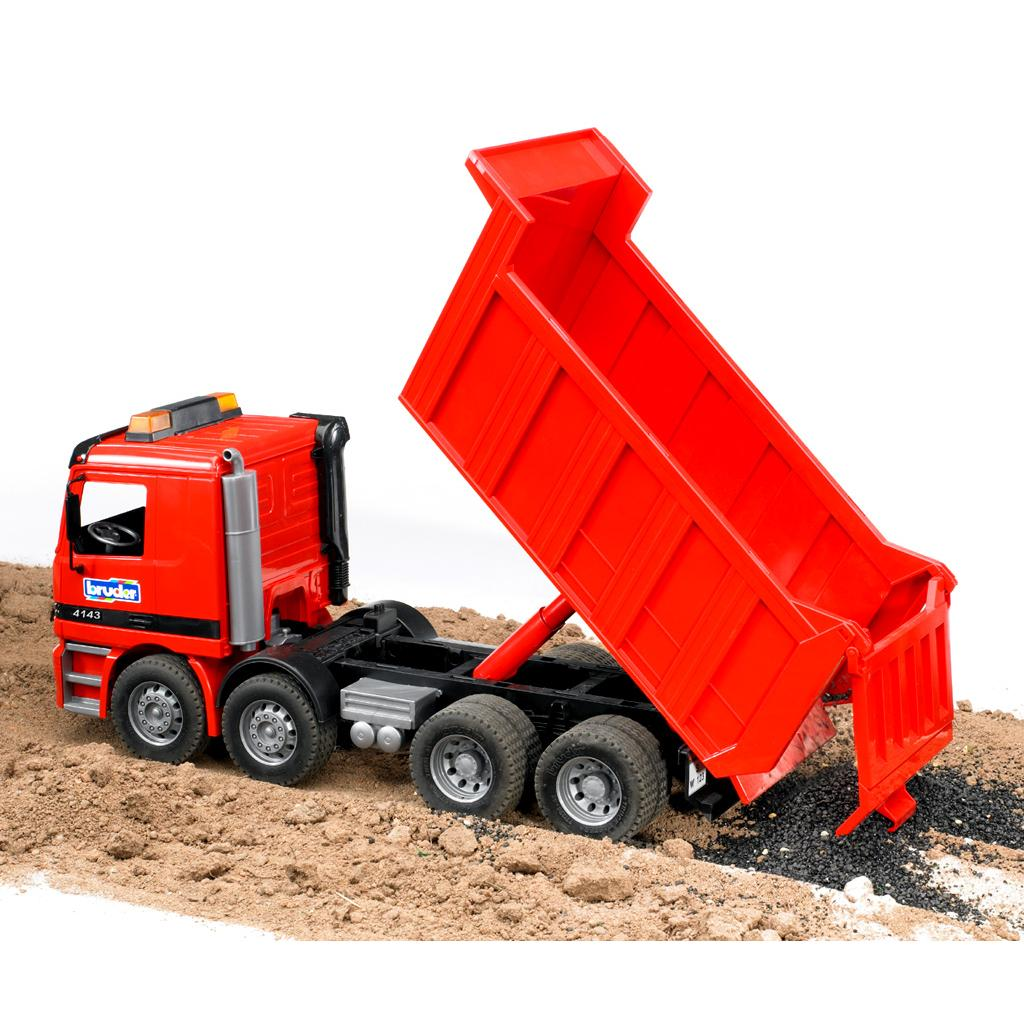
\includegraphics[width=\linewidth]{img/camion-benne.jpg}
\caption{Camion benne en extension}
\label{fig:image3}
\end{center}
\end{minipage}
\hfill
\begin{minipage}[c]{.48\linewidth}
Soit $R_O(\overrightarrow{x_0},\overrightarrow{y_0},\overrightarrow{z_0})$ un repère lié au châssis 0 d'un camion benne.
Soient $R_1(\overrightarrow{x_1},\overrightarrow{y_1},\overrightarrow{z_1})$ un repère lié à la benne 1 et $R_2(\overrightarrow{x_2},\overrightarrow{y_2},\overrightarrow{z_2})$ un repère lié à la tige 2
et au corp 3 du vérin hydraulique.

Le mécanisme étudié est considéré dans le plan $(\overrightarrow{x_0},\overrightarrow{y_0})$. Le corps 1 a un mouvement de rotation d'axe $(O, \overrightarrow{z_0})$ par rapport au châssis 0 avec $\alpha=(\overrightarrow{x_0},\overrightarrow{x_1})=(\overrightarrow{y_0},\overrightarrow{y_1})$. La tige 2 à un mouvement de rotation d'axe $(B, \overrightarrow{z_0})$ par rapport à la benne 1 et le corp 3 du vérin un mouvement de rotation d'axe $(A, \overrightarrow{z_0})$ par rapport au châssis 0 du camion benne.

La tige 2 a un mouvement de translation rectiligne de direction $\overrightarrow{y_2}$ par rapport au corps 3 du vérin. On pose $\overrightarrow{AB}=\lambda.\overrightarrow{y_2}$ ($\lambda$ varie).
\end{minipage}
\end{figure}

Seul le mouvement de rotation de la benne 1 par rapport au chassis 0 sera considéré.

\paragraph{Question 1:} Dans un premier temps, l'étude portera sur un mouvement dont l'accélération sera de la forme:

\begin{itemize}
 \item Pour $0 \le t \le t_0/2$ : $\ddot{\theta(t)}=\ddot{\theta_0}.t$,
 \item Pour $t_0/2 \le t \le t_0$ : $\ddot{\theta(t)}=\ddot{\theta_0}.(t_0-t)$,
 \item Pour $t_0 \le t \le T-t_0$ : $\ddot{\theta(t)}=0$,
 \item Pour $T-t_0 \le t \le T-t_0/2$ : $\ddot{\theta(t)}=\ddot{\theta_0}.(T-t_0-t)$,
 \item Pour $T-t_0/2 \le t \le T$ : $\ddot{\theta(t)}=\ddot{\theta_0}.(t-T)$.
 \item Les conditions initiales étant: $\dot{\theta(0)}=0$ et $\theta(0)=0$. $\ddot{\theta_0}$ est une constante.
\end{itemize}

Tracer:
\begin{itemize}
 \item l'accélération $\ddot{\theta(t)}$ en fonction du temps (t),
 \item la vitesse $\dot{\theta(t)}$ en fonction du temps (t),
 \item la position $\theta(t)$ en fonction du temps (t).
\end{itemize}

\newpage

\paragraph{Question 2:} Dans un second temps, la valeur pilotée sera la vitesse, elle sera de la forme:

\begin{itemize}
 \item Pour $0 \le t \le t_0$ : $\dot{\theta(t)}=\frac{\dot{\theta_0}}{t_0}.t$,
 \item Pour $t_0 \le t \le T-2.t_0$ : $\dot{\theta(t)}=\dot{\theta_0}$,
 \item Pour $T-2.t_0 \le t \le T$ : $\dot{\theta(t)}=-\frac{\dot{\theta_0}}{2.t_0}.t+\frac{\dot{\theta_0}}{2.t_0}.T$,
 \item Les conditions initiales étant: $\dot{\theta(0)}=0$ et $\theta(0)=0$. $\dot{\theta_0}$ est une constante.
\end{itemize}

Tracer:
\begin{itemize}
 \item la vitesse $\dot{\theta(t)}$ en fonction du temps (t),
 \item l'accélération $\ddot{\theta(t)}$ en fonction du temps (t),
 \item la position $\theta(t)$ en fonction du temps (t).
\end{itemize}

~\

\newpage

\section{Bras manipulateur}

Un bras manipulateur est le bras d'un robot généralement programmable, avec des fonctions similaires à un bras humain. Les liens de ce manipulateur sont reliés par des axes permettant, soit du mouvement de rotation (comme dans un robot articulé) ou de translation (linéaire) de déplacement.

\begin{figure}[htbp]
\begin{minipage}[c]{.48\linewidth}
\begin{center}
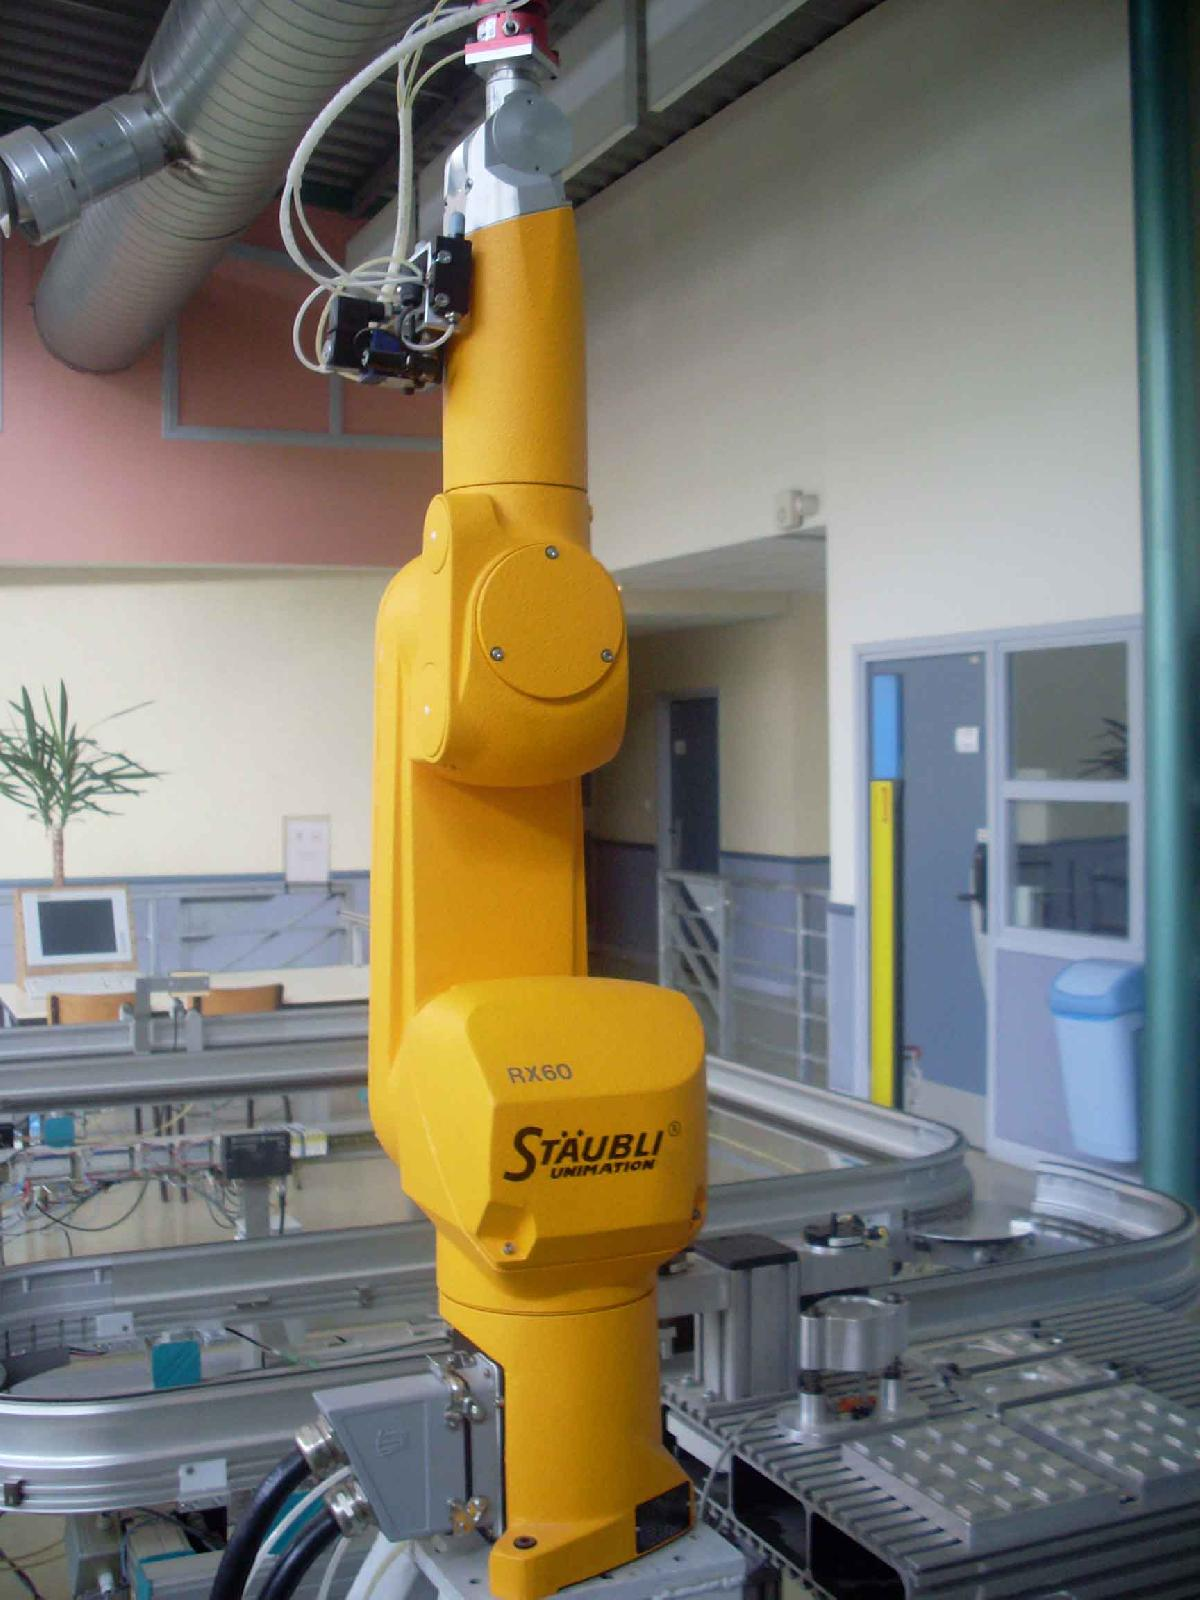
\includegraphics[width=\linewidth]{img/robot.jpg}
\caption{Exemple de bras manipulateur}
\label{fig:image4}
\end{center}
\end{minipage}
\hfill
\begin{minipage}[c]{.48\linewidth}
\begin{center}
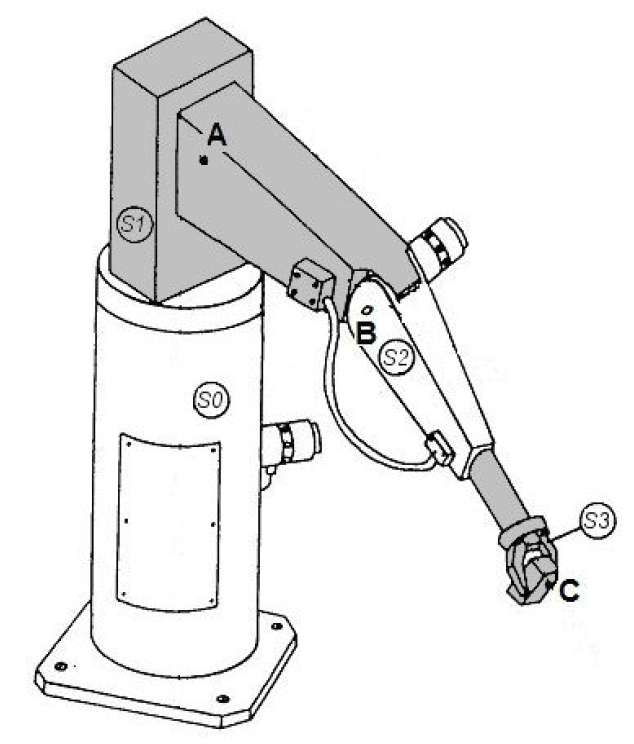
\includegraphics[width=\linewidth]{img/bras.png}
\caption{Bras étudié}
\label{fig:image5}
\end{center}
\end{minipage}
\end{figure}

Le schéma de droite ci-dessus représente un bras manipulateur permettant de déplacer des objets.
Ce mécanisme est constitué de :
\begin{itemize}
 \item Un bâti S0,
 \item Un solide S1 entraîné en rotation par un moteur M1,
 \item Un solide S2 entraîné en rotation par un moteur M2,
 \item Un solide S3 entraîné en translation par un vérin V1,
 \item Une pince située à l'extrémité du vérin permettant de saisir l'objet.
\end{itemize}

\begin{itemize}
 \item Le mouvement de S1 par rapport à S0 est une rotation d'axe $(A, \overrightarrow{z_0})$, 
 \item Le mouvement de S2 par rapport à S1 est une rotation d'axe $(B, \overrightarrow{x_1})$,
 \item Le mouvement de S3 par rapport à S2 est une translation rectiligne de direction $\overrightarrow{z_2}$.
\end{itemize}

On pose $\overrightarrow{AB}=a.\overrightarrow{y_1}$ (a étant une constante).


Seul le mouvement de translation de S3 par rapport à S2 sera considéré.

\newpage

\paragraph{Question 1:} Dans un premier temps, l'étude portera sur un mouvement dont l'accélération sera de la forme:

\begin{itemize}
 \item Pour $0 \le t \le t_0$ : $\ddot{x(t)}=\ddot{x_0}.sin(\frac{\pi.t}{t_0})$,
 \item Pour $t_0 \le t \le t_0+t_1$ : $\ddot{x(t)}=0$,
 \item Pour $t_0+t_1 \le t \le 2.t_0+t_1$ : $\ddot{x(t)}=-\ddot{x_0}.sin(\frac{\pi}{t_0}(t-(t_0+t_1)))$,
 \item Les conditions initiales étant: $\dot{x(0)}=0$ et $x(0)=0$. $\ddot{x_0}$ est une constante.
\end{itemize}

Tracer:
\begin{itemize}
 \item l'accélération $\ddot{x(t)}$ en fonction du temps (t),
 \item la vitesse $\dot{x(t)}$ en fonction du temps (t),
 \item la position $x(t)$ en fonction du temps (t).
\end{itemize}

\paragraph{Question 2:} Dans un second temps, la valeur pilotée sera la vitesse, elle sera de la forme:

\begin{itemize}
 \item Pour $0 \le t \le t_0$ : $\dot{x(t)}=\frac{\dot{x_0}}{t_0}.t$,
 \item Pour $t_0 \le t \le t_0+T$ : $\dot{x(t)}=\dot{x_0}$,
 \item Pour $t_0+T \le t \le t_0+T+t_1$ : $\dot{x(t)}=-\frac{\dot{x_0}}{t_1}.t+\frac{\dot{x_0}}{t_1}.(T+t_0+t_1)$,
 \item Les conditions initiales étant: $\dot{x(0)}=0$ et $x(0)=0$.  $\dot{x_0}$ est une constante.
\end{itemize}

Tracer:
\begin{itemize}
 \item la vitesse $\dot{x(t)}$ en fonction du temps (t),
 \item l'accélération $\ddot{x(t)}$ en fonction du temps (t),
 \item la position $x(t)$ en fonction du temps (t).
\end{itemize}


\end{document}